%!TEX root = lec05_query_processing.tex

%
% -------------------------------------------
%
\newsavebox\iteratorExampleTree
\savebox{\iteratorExampleTree}{
\begin{tikzpicture}[semithick,align=center,node distance=0.875cm,every node/.style={inner sep=1,outer sep=1,font=\footnotesize}]
% \node (0) at (0,0) {} ; %empty node with ``answer''
\node (1) at (0,0) {$\pi_{\texttt{role,imdb}}$};
\node (3) [below of= 1] {$\Join$};
\node (4) [below left of= 3, xshift=-0.25cm] {\lstinline[style=SQL]!scan(Movie)!};
\node (2) [below right of= 3, xshift=0.25cm, yshift=-0.75cm] {$\sigma_{\texttt{actor='Bill Murray'}}$};
\node (5) [below of =2] {\lstinline[style=SQL]!scan(Cast)!};
\path[->]
    (4) edge (3)
    (5) edge (2) 
    (3) edge (1)
    (2) edge (3);
    % (1) edge (0);
\end{tikzpicture}
}

%
% -------------------------------------------
%
\begin{frame}{The Iterator Interface}

All nodes in a query plan must implement the following three methods:


\begin{columns}[onlytextwidth]
\begin{column}{0.6\textwidth}
\begin{itemize}[label=$\circ$]
\item \textbf{Open()}:  creates/requests the necessary data structures.
\item \textbf{GetNext()}:  produces \alert{\textbf{the} next tuple} for that node.
\item \textbf{Close()}:  releases the necessary data structures.
\end{itemize}


\end{column}
\begin{column}{0.4\textwidth}
\flushright
\usebox\iteratorExampleTree
\end{column}
\end{columns}

\vskip1em

\begin{block}{\alert{\textbf{Remember this}}}
Each call to \textbf{GetNext()} \alert{produces just one tuple}: the next tuple that the node must return.
\end{block}

\end{frame}


%
% -------------------------------------------
%
\begin{frame}{Open()/Close()}
\vskip1em
\begin{columns}[onlytextwidth]
\begin{column}{0.6\textwidth}
\textbf{Open()} is called recursively, top-down, from the root of the tree

\vskip0.5em

A call to \textbf{Open()} is supposed to:

\vskip0.5em

\begin{enumerate}[label=(\arabic*)]
\item create any necessary input buffers
\item initialize any variables needed (ex: pointers to tuples in a nested loop join operator)
\item open a file if the operator is a table or index scan
\end{enumerate}

\vskip1em

The analogous \textbf{Close()} method frees up all those resources.

\end{column}
\begin{column}{0.4\textwidth}
\qquad\qquad
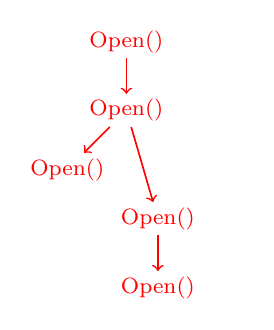
\begin{tikzpicture}[semithick,align=center,node distance=0.875cm,every node/.style={inner sep=1,outer sep=1,font=\footnotesize}]
\node[anchor=north,inner sep=0pt,outer sep=0pt] at (0,0) {\scalebox{1}{\usebox{\iteratorExampleTree}}};

\node (0) at (-1.5,-0.125) [color=red] {Open()};
\pause
\node (1) [below of=0,color=red] {Open()};
\draw [->, color=red] (0) -- (1);
\pause
\node (2) [below of=1,xshift=-0.75cm,yshift=0.125cm,,color=red] {Open()};
\draw [->, color=red] (1) -- (2);
\pause
\node (3) [below of=1,xshift=0.4cm, yshift=-0.5cm,color=red] {Open()};
\draw [->, color=red] (1) -- (3);
\pause
\node (4) [below of=3,color=red] {Open()};
\draw [->, color=red] (3) -- (4);
\end{tikzpicture}
\end{column}
\end{columns}

\end{frame}


%
% -------------------------------------------
%
\begin{frame}{GetNext()}

\vskip1em

\begin{columns}[onlytextwidth]
\begin{column}{0.55\textwidth}

\textbf{GetNext()} computes \alert{one more tuple} and returns it to the operator ``above'' it in the plan.

\vskip1em

\textbf{GetNext()} returns \alert{\lstinline[style=SQL]{<EOF>}} when there are no more tuples to return.

\end{column}
\begin{column}{0.4\textwidth}
\flushright
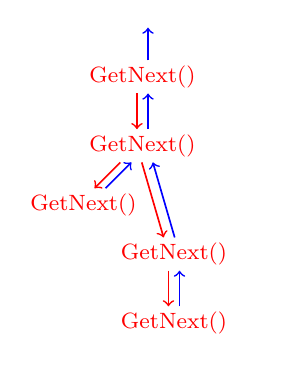
\begin{tikzpicture}[semithick,align=center,node distance=0.875cm,every node/.style={inner sep=1,outer sep=1,font=\footnotesize}]
\node[anchor=north,inner sep=0pt,outer sep=0pt] at (0,0) {\scalebox{1}{\usebox{\iteratorExampleTree}}};
\node (0) at (-1.5,-0.125) [color=red] {GetNext()};
\pause
\node (1) [below of=0,color=red] {GetNext()};
\draw [->, color=red,transform canvas={xshift=-2pt}] (0) -- (1);
\pause
\node (2) [below of=1,xshift=-0.75cm,yshift=0.125cm,,color=red] {GetNext()};
\draw [->, color=red,transform canvas={xshift=-2pt}] (1) -- (2);
\pause
\draw [->,color=blue,transform canvas={xshift=2pt}] (2) -- (1);
\pause
\node (3) [below of=1,xshift=0.4cm, yshift=-0.5cm,color=red] {GetNext()};
\draw [->, color=red,transform canvas={xshift=-2pt}] (1) -- (3);
\pause
\node (4) [below of=3,color=red] {GetNext()};
\draw [->, color=red,transform canvas={xshift=-2pt}] (3) -- (4);
\pause
\draw [->,color=blue,transform canvas={xshift=2pt}] (4) -- (3);
\pause
\draw [->,color=blue,transform canvas={xshift=2pt}] (3) -- (1);
\pause
\draw [->,color=blue,transform canvas={xshift=2pt}] (1) -- (0);
\pause
\draw [->,color=blue,transform canvas={xshift=2pt}] (0) -- (-1.5,0.5);
\end{tikzpicture}
\end{column}
\end{columns}

\end{frame}

\begin{frame}
\begin{columns}[onlytextwidth]
\begin{column}{0.6\textwidth}
\alert{scan(R)}: returns next tuple from $R$, reading a new block from disk if needed.

\vskip2em

\alert{$\pi_{a_1,\ldots,a_n}(R)$}: calls \lstinline[style=SQL]{getNext()} on operator below, strip unwanted attributes and return the resulting tuple
\end{column}
\begin{column}{0.4\textwidth}
\flushright
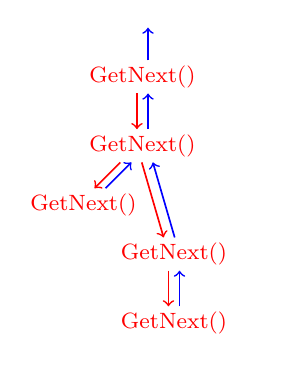
\begin{tikzpicture}[semithick,align=center,node distance=0.875cm,every node/.style={inner sep=1,outer sep=1,font=\footnotesize}]
\node[anchor=north,inner sep=0pt,outer sep=0pt] at (0,0) {\scalebox{1}{\usebox{\iteratorExampleTree}}};
\node (0) at (-1.5,-0.125) [color=red] {GetNext()};
\node (1) [below of=0,color=red] {GetNext()};
\draw [->, color=red,transform canvas={xshift=-2pt}] (0) -- (1);
\node (2) [below of=1,xshift=-0.75cm,yshift=0.125cm,,color=red] {GetNext()};
\draw [->, color=red,transform canvas={xshift=-2pt}] (1) -- (2);
\draw [->,color=blue,transform canvas={xshift=2pt}] (2) -- (1);
\node (3) [below of=1,xshift=0.4cm, yshift=-0.5cm,color=red] {GetNext()};
\draw [->, color=red,transform canvas={xshift=-2pt}] (1) -- (3);
\node (4) [below of=3,color=red] {GetNext()};
\draw [->, color=red,transform canvas={xshift=-2pt}] (3) -- (4);
\draw [->,color=blue,transform canvas={xshift=2pt}] (4) -- (3);
\draw [->,color=blue,transform canvas={xshift=2pt}] (3) -- (1);
\draw [->,color=blue,transform canvas={xshift=2pt}] (1) -- (0);
\draw [->,color=blue,transform canvas={xshift=2pt}] (0) -- (-1.5,0.5);\end{tikzpicture}
\end{column}
\end{columns}
\end{frame}


%
% -------------------------------------------
%
\begin{frame}
\begin{columns}[onlytextwidth]
\begin{column}{0.6\textwidth}
\alert{$\sigma_{C}(R)$}: \underline{repeatedly} calls \lstinline[style=SQL]{getNext()} on operator below until a tuple that satisfies the condition $C$ is found; returning that tuple (or \lstinline[style=SQL]{<EOF>} if no such tuple exists).

\vskip2em

\alert{$R \Join_{C} S$}: calls \lstinline[style=SQL]{getNext()} on iterators for $R$ and $S$ according to the algorithm, until a match is found.

\end{column}
\begin{column}{0.4\textwidth}
\flushright
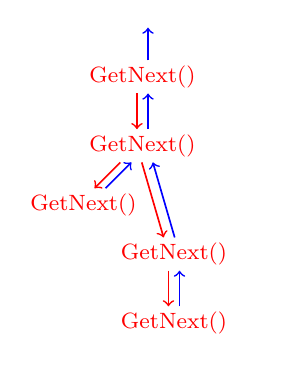
\begin{tikzpicture}[semithick,align=center,node distance=0.875cm,every node/.style={inner sep=1,outer sep=1,font=\footnotesize}]
\node[anchor=north,inner sep=0pt,outer sep=0pt] at (0,0) {\scalebox{1}{\usebox{\iteratorExampleTree}}};
\node (0) at (-1.5,-0.125) [color=red] {GetNext()};
\node (1) [below of=0,color=red] {GetNext()};
\draw [->, color=red,transform canvas={xshift=-2pt}] (0) -- (1);
\node (2) [below of=1,xshift=-0.75cm,yshift=0.125cm,,color=red] {GetNext()};
\draw [->, color=red,transform canvas={xshift=-2pt}] (1) -- (2);
\draw [->,color=blue,transform canvas={xshift=2pt}] (2) -- (1);
\node (3) [below of=1,xshift=0.4cm, yshift=-0.5cm,color=red] {GetNext()};
\draw [->, color=red,transform canvas={xshift=-2pt}] (1) -- (3);
\node (4) [below of=3,color=red] {GetNext()};
\draw [->, color=red,transform canvas={xshift=-2pt}] (3) -- (4);
\draw [->,color=blue,transform canvas={xshift=2pt}] (4) -- (3);
\draw [->,color=blue,transform canvas={xshift=2pt}] (3) -- (1);
\draw [->,color=blue,transform canvas={xshift=2pt}] (1) -- (0);
\draw [->,color=blue,transform canvas={xshift=2pt}] (0) -- (-1.5,0.5);\end{tikzpicture}
\end{column}
\end{columns}
\end{frame}

%
% -------------------------------------------
%
\begin{frame}{Iterators for other binary operators}

The iterators for \alert{$R - S$}, \alert{$R \cup S$} and \alert{$R \cap S$} are analogous to \alert{$R \Join_{C} S$} and make repeated calls to \lstinline[style=SQL]{getNext()} on the iterators for $R$ and $S$ to obtain tuples from each sub-expression.

\vskip2em

We will look at intricacies of the algorithms later in these slides.


\end{frame}


%
% -------------------------------------------
%
\begin{frame}[fragile]

The next slides show naive (and incomplete) Python-like implementations of some of the iterators, focusing on semantics\footnote{After we look at the I/O cost analysis of simple query plans, we will discuss better algorithms for the iterators.} but omitting details. 

\vskip1em

Assume there is an interface, called \lstinline[style=Python]{Iterator}, declaring all operations that each iterator must implement.
\begin{itemize}[-,topsep=-5pt,noitemsep]
\item For simplicity, we omit details like constructors.
\item \lstinline[style=Python]{Iterator.from(X)} compiles relational expression \lstinline[style=Python]{X} into the appropriate iterator object.
\end{itemize}

\vskip1em



\end{frame}

%
% -------------------------------------------
%
\begin{frame}[fragile]{Iterator for $\sigma_C(R)$ }

\begin{lstlisting}[style=Python,multicols=2]
Class Selection(Iterator):

  def Open():
    self.i = Iterator.from(self.R)
    self.i.Open()


  def Close():
    self.i.Close()


  def GetNext():
    # read tuple from R
    t = self.i.GetNext() 
    while t !=  EOF and 
        not satisfies(t, self.C):
      t = i.GetNext()
    yield t

\end{lstlisting}


\vskip0.25em

\begin{block}{}%{Iterator state}
The selection condition (\lstinline[style=Python]{self.C}) is an instance variable\footnotemark ~because each selection in the plan has its own condition.

Also, \lstinline[style=Python]{self.i} refers to another iterator, corresponding to the sub-plan ``below'' that selection.
\end{block}

\vskip1em

\footnotetext{\url{https://www.digitalocean.com/community/tutorials/understanding-class-and-instance-variables-in-python-3}}
\end{frame}



%
% -------------------------------------------
%
\begin{frame}[fragile]{Iterator for $\pi_{a_1,\ldots,a_n}(R)$}

\begin{lstlisting}[style=Python,multicols=2]
Class Projection(Iterator):

  def Open():
    self.i = Iterator.from(self.R)
    self.i.Open()


  def Close():
    self.i.Close()




  def GetNext():
    # read tuple from R
    t = self.i.GetNext() 
    if t == EOF:
      yield EOF
    else:
      # remove unwanted attributes
      yield (t.a1, ... , t.an)

\end{lstlisting}

\end{frame}

%
% -------------------------------------------
%
\begin{frame}[fragile]{Iterator for \lstinline[style=SQL]{scan(R)} on a table file}
\label{table_scan_iterator}

\begin{lstlisting}[style=Python,multicols=2]
Class Scan(Iterator):

  def Open():
    self.F = File.open(self.R)
    self.b = F.first_block()
    self.t = b.first_tuple()
    

  def Close():
    self.F.Close()





  def GetNext():
    if self.t is None:
      self.b = self.F.next_block()
      if self.b is None:
        yield EOF
      else:
        self.t = self.b.first_tuple()

    old = self.t
    self.t = self.b.next_tuple()
    yield old
\end{lstlisting}


\vskip0,5em

\begin{block}{The state of a table scan}
\lstinline[style=Python]{self.b} and \lstinline[style=Python]{self.t} represent the \textbf{state} of the iterator, and always refer to the tuple that should be returned next.
\end{block}

\end{frame}

%
% ------------------------------------
%

\newsavebox{\UnionAllIteratorCode}
\begin{lrbox}{\UnionAllIteratorCode}
\begin{minipage}{\textwidth}
\begin{lstlisting}[style=Python,multicols=2]
Class Union_All(Iterator):

  def Open():
    self.i = Iterator.from(self.R)
    self.i.Open()
    self.reading_R = true


  def Close():
    self.i.Close()




  def GetNext():
    t = self.i.GetNext()
    if t == EOF:
      if reading_R: 
        self.i.close()
        self.i = Iterator.from(self.S)
        self.i.Open()
        yield self.i.GetNext()
    else:
      yield EOF
\end{lstlisting}
\end{minipage}
\end{lrbox}

\begin{frame}[fragile]{Iterator for bag version of $R \cup S$ (\lstinline[style=SQL]{UNION ALL})}

\hspace*{-1.25em}\usebox{\UnionAllIteratorCode}


\vskip1em

\begin{block}{No need for duplicate detection}
Return all of $R$ first, then all of $S$ (\lstinline[style=Python]{self.reading_R} tells which one we're reading from).
\end{block}

\end{frame}



%
% ------------------------------------
%

\newsavebox\CrossProductIterator
\begin{lrbox}{\CrossProductIterator}
\begin{minipage}{\textwidth}
\begin{lstlisting}[style=Python,multicols=2]
Class Cross_Product(Iterator):

  def Open():
    self.i = Iterator.from(self.R)
    self.i.Open()
    self.j = Iterator.from(self.S)
    self.j.Open()
    self.t_i = self.i.GetNext()


  def Close():
    self.i.Close()
    self.j.Close()



  def GetNext():
    if self.t_i != EOF:
      t_j = self.j.GetNext()
      if t_j != EOF:
        t = concatenate(self.t_i, t_j)
        yield t
      else:
        self.t_i = self.i.GetNext()
        Iterator.rewind(self.j)
        yield this.GetNext()
    else:
      yield EOF
\end{lstlisting}
\end{minipage}
\end{lrbox}

\begin{frame}[fragile]{Iterator for $R \times S$ using nested loops}
\label{cross_product_iterator}

\hspace*{-1.5em}\usebox\CrossProductIterator

\begin{block}{Rewind?}
Every time we advance to a new tuple of $R$ we rewind the iterator on $S$ back to the start!
\end{block}

\end{frame}


%
% ------------------------------------
%

\newsavebox\NLJoinIterator
\begin{lrbox}{\NLJoinIterator}
\begin{minipage}{\textwidth}
\begin{lstlisting}[style=Python,multicols=2]
Class Nested_Loop_Join(Iterator):

  def Open():
    self.i = Iterator.from(self.R)
    self.i.Open()
    self.j = Iterator.from(self.S)
    self.j.Open()
    self.t_i = self.i.GetNext()


  def Close():
    self.i.Close()
    self.j.Close()






  def GetNext():
    if self.t_i != EOF:
      t_j = self.j.GetNext()
      if t_j != EOF:
        t = join(self.t_i, t_j)
        if satisfies(t, self.C):
          yield t
        else:
          yield this.GetNext()  
      else:
        self.t_i = self.i.GetNext()
        Iterator.rewind(self.j)
        yield this.GetNext()
    else:
      yield EOF
\end{lstlisting}
\end{minipage}
\end{lrbox}

\begin{frame}[fragile]{Iterator for $R \Join_C S$ using nested loops}
\label{nested_loop_join_iterator}

\usebox\NLJoinIterator


\end{frame}


%
% ------------------------------------
%
\begin{frame}[fragile]{Iterator for \lstinline[style=SQL]{distinct(R)} (duplicate elimination)}
\label{distinct_iterator}

\begin{lstlisting}[style=Python,multicols=2,mathescape]
Class Distinct(Iterator):

  def Open():
    self.i = Iterator.from(self.R)
    self.i.Open()
    self.s = set() # hash set

  def Close():
    self.i.Close()
    self.s = None




  def GetNext():
    # read tuple from R
    t = self.i.GetNext() 
    while t != EOF and t in self.s:
      t = self.i.GetNext() 
    yield t


$\,$
\end{lstlisting}

\vskip0.5em

\begin{block}{Duplicate elimination with an in-memory set}
To make sure we never repeat a tuple, we can keep every tuple that is ever returned in a set (\lstinline[style=Python]{self.s}) in memory.
\end{block}
\end{frame}

%
% ------------------------------------
%
\begin{frame}{Implementation considerations}

Again, the previous slides are meant to give you \alert{\textbf{the intuition}} of the code for an iterator. 

There are many practical considerations that are too low level to list in the notes. For example, for the \lstinline[style=SQL]{distinct()} iterator (slide~\ref{distinct_iterator}), the DBMS may have to \alert{keep the a hash set on disk}, depending on the system load at query execution time!

Similarly for joins (and most other binary operators), the DBMS chooses the actual algorithm and data structure to use in real-time, based on the resources (especially RAM) available.

\end{frame}